%\documentclass[12pt,a4paper,notitlepage,fleqn,twoside]{book}		% Zweiseitiger Druck
%\documentclass[12pt,a4paper,notitlepage,fleqn,oneside]{book}		% Einseitiger Druck
%\documentclass[12pt,a4paper,notitlepage,twoside]{book}		        % Zweiseitiger Druck, Formeln zentriert
\documentclass[12pt,a4paper,notitlepage,oneside]{book}		        % Einseitiger Druck, Formeln zentriert


%%%%%%%%%%%%%%%%%%%%%%%%%%%%%%%%%%%%%%%%%%%%%%%%%%%%%%%%%%%%%%%%%%%%%%%%%%%%%%%%%%%%%%%%%%%%%%%%%%%%%%%%
%%%   Layout - DO NOT CHANGE              	                                                         %%%
%%%%%%%%%%%%%%%%%%%%%%%%%%%%%%%%%%%%%%%%%%%%%%%%%%%%%%%%%%%%%%%%%%%%%%%%%%%%%%%%%%%%%%%%%%%%%%%%%%%%%%%%

% Ein- oder zweiseitiger Druck - Documentclass oben entsprechend anpassen!
%\newcommand{\Drucklayout}{Einseitig}
%\newcommand{\Drucklayout}{Zweiseitig}

% Fuer serifenlose Schrift folgendes einkommentieren
\newcommand{\Schriftart}{serifenlos}
%\newcommand{\Schriftart}{LaTeX-Standard}

% Ausrichtung der Formeln linksbuendig oder zentriert - Documentclass oben entsprechend anpassen!
%\newcommand{\Formelausrichtung}{links}
%\newcommand{\Formelausrichtung}{zentriert}

% Verzeichnisse im Inhaltsverzeichnis auffuehren
\newcommand{\preChapterToC}{ja}


%%%%%%%%%%%%%%%%%%%%%%%%%%%%%%%%%%%%%%%%%%%%%%%%%%%%%%%%%%%%%%%%%%%%%%%%%%%%%%%%%%%%%%%%%%%%%%%%%%%%%%%%
%%%   Packages, eigene Makros und Formatdefinitionen                                                 %%%
%%%%%%%%%%%%%%%%%%%%%%%%%%%%%%%%%%%%%%%%%%%%%%%%%%%%%%%%%%%%%%%%%%%%%%%%%%%%%%%%%%%%%%%%%%%%%%%%%%%%%%%%

	
\usepackage[english]{babel} 	% Sprachpaket
% \usepackage[latin1]{inputenc} 		% Konvertierungspaket (Sprachen:Westeuropa)
\usepackage[utf8]{inputenc} 		% joba Konvertierungspaket (Sprachen:Westeuropa)

\usepackage{ifthen}		% if then
\usepackage[scaled=0.92]{helvet}
\ifthenelse{\equal{\Schriftart}{serifenlos}}{
	\renewcommand{\sfdefault}{phv}
	\renewcommand{\familydefault}{\sfdefault}	
}{}

% Anfuehrungszeichen
\usepackage[autostyle=true,german=quotes]{csquotes}

\usepackage[centertags]{amsmath}		% Mathepakete
\usepackage{amssymb}
\usepackage{fdsymbol}

%\usepackage[pdftex]{graphicx}
%\usepackage{epstopdf}
%\usepackage{eso-pic}
\usepackage{pstool}


\usepackage[absolute]{textpos}

\usepackage[format=hang, font=footnotesize, labelfont=bf]{caption}  % Layout fuer Bildbeschriftung

\usepackage{fancyhdr}	% Definition von Kopf- und Fusszeilen

\usepackage{xcolor}		% fuer farbige Texte und Tabellen (RGB-Farbraum)

\usepackage{calc}

\ifthenelse{\equal{\preChapterToC}{ja}}{
	\usepackage[nottoc]{tocbibind}
}{
	\usepackage[nottoc,notlof,notlot]{tocbibind}
}
\usepackage[titles]{tocloft}	% Package zum Bearbeiten des Layouts des Abbildungs- und Tabellenverzeichnisses
\usepackage{titletoc}	% Package zum Bearbeiten des Layouts des Inhaltsverzeichnisses

\normalsize

%-----------------------------------------------------------------------------------------------------------%

\usepackage[resetlabels,labeled]{multibib}		% mehrere Bibliographien

\usepackage[rigidchapters]{titlesec}

\usepackage{textcomp}

\usepackage[labelformat=simple]{subcaption}	% Subcaptions

\usepackage{enumitem} % Aufzaehlungen

\usepackage{multirow}	% Multirow - Tabellen
\usepackage{longtable}	% Lange Tabelle
\usepackage{array}
\usepackage{booktabs}

%\usepackage{color}		% fuer Farben im allgemeinen
\usepackage{colortbl}	% fuer die Hintergrundfarbe einzelner Zellen in Tabellen
\usepackage{ragged2e}

\usepackage{url}		% URL-Package

\usepackage{nomencl}	% Abkuerzungen und Verzeichnisse
\usepackage{makeidx}	% Index erstellen

\usepackage{blindtext}	% Lorem ipsum

\usepackage{setspace}	% Zeilenabstand

\usepackage[bottom]{footmisc}	% Fussnotenposition
\usepackage{chngcntr}

\usepackage{pdfpages}

%\usepackage{showframe}% zum Anzeigen des Seitenlayouts

\usepackage{lipsum} %Blindtext

\usepackage[]{hyperref}	% Links usw.

\usepackage{titlesec} % Space before heading




				    % Notwendige Packete
	
% Makros

\newcommand{\TODO}[1]{{\color{red} #1}}
\newcommand{\EVTL}[1]{{\color{blue} #1}}


\newcommand{\VECSYM}[1]{\boldsymbol{#1}}			% Symbol als Vektor (fett)
\newcommand{\VEC}[1]{\mathbf{#1}}					% Vektor (fett)
\newcommand{\sign}[1]{\mbox{sign}\left\{#1\right\}}	% Signum-Funktion
\newcommand{\intd}{\textnormal{\;d}}				% d bei einem Integral
\newcommand{\ind}[1]{_\textnormal{#1}}				% konstanter Index in Matheumgebung (nicht kursiv)
\newcommand{\einheit}[1]{\,\textnormal{#1}}			% Einheit in Matheumgebung (nicht kursiv)
\newcommand{\const}[1]{\textnormal{#1}}				% Konstante in Matheumgebung (nicht kursiv)
\newcommand{\prozent}{\,\%}		% Prozent im Mathemodus


% Begriffe hervorheben
\newcommand{\significant}[1]{{\bf #1}}
\newcommand{\english}[1]{\emph{(engl. #1)}}

% Name
\newcommand{\name}[1]{\textsc{#1}}

% Abkuerzungs- und Symbolverzeichnis
\newcommand{\abk}[2]{({#1})\nomenclature[A]{#1}{#2}}
%\abk{Abkuerzung}{ausgeschrieben}

\newcommand{\sym}[3]{{#1}\nomenclature[S,#2]{#1}{#3}}		% Sortierung eingefuegt
%\sym{Symbol}{Sortierung}{Symbolbezeichnung}

% Referenzen fuer Formeln
\newcommand{\glg}[1]{Gleichung~\eqref{#1}}
% Referenzen fuer Abbildung
\newcommand{\abb}[1]{Abbildung~\ref{#1}}
% Referenzen fuer Tabellen
\newcommand{\tab}[1]{Tabelle~\ref{#1}}


% Farben
\definecolor{dunkelgrau}{rgb}{0.8,0.8,0.8}
\definecolor{hellgrau}{rgb}{0.9,0.9,0.9}
\definecolor{fapsgruen}{RGB}{151,193,57}
\definecolor{fapsblau}{RGB}{41,97,147}
\definecolor{fapsgraudunkel}{RGB}{95,95,95}


% Angaben fuer Literaturverzeichnis
\newcommand{\bblin}{in}
\newcommand{\bblvolume}{Vol.}
\newcommand{\bbledition}{Auflage}
\newcommand{\bbleditor}{Hrsg.}
\newcommand{\bbleditors}{Hrsg.}
\newcommand{\bblseries}{aus der Reihe}
\newcommand{\bblpp}{S.}
\newcommand{\bblaccess}{Aufgerufen am}

% Rechts- und linksbuendige Spalten mit fester Breite
\newcolumntype{R}[1]{>{\RaggedLeft\arraybackslash}p{#1}}
\newcolumntype{L}[1]{>{\RaggedRight\arraybackslash}p{#1}}
\newcolumntype{C}[1]{>{\centering\arraybackslash}p{#1}}

% Abstand der Punkte im Inhaltsverzeichnis / wenn keine Punkte, dann 0pc
\newcommand{\vzPunkte}{\titlerule*[1pc]{.}}

% Abstand zwischen Zeilen
\renewcommand{\arraystretch}{1.5}					% Selbstdefinierte Befehle
	% Offset zur einfacheren Abstandsangabe (Papier links oben ist 'Null')
\setlength{\hoffset}{-1.15cm}
\setlength{\voffset}{0cm}

% Kopfzeile
\headheight.7cm		% Hoehe vom Header

% Textfeld
\textheight24.2cm
\textwidth16cm

% Layout vertikale Abstaende
\headsep1.1cm															% Abstand Header - Text
\setlength{\topmargin}{-1in + 1.2cm}			                        % Abstand oberer Seitenrand - Header
\setlength{\footskip}{1.5cm}							                   % Abstand Text - Fusszeile

% Layout horizontale Abstaende gerade Seiten
\setlength{\evensidemargin}{0cm}										% Abstand linker Seitenrand zum Textrand
% Layout horizontale Abstaende ungerade Seiten
\ifthenelse{\boolean{@twoside}}{
	\setlength{\oddsidemargin}{-\evensidemargin}						% Abstand rechter Seitenrand zum Textrand
}{}

% Notizbereiche
%\setlength{\marginparwidth}{0cm}
%\marginparsep8pt


%% Fuss- und Kopfzeilenformatierung
\pagestyle{fancy}
%\renewcommand{\chaptermark}[1]{ \markboth{\MakeUppercase{\thechapter\; #1}}{} }
%\renewcommand{\sectionmark}[1]{ \markright{\MakeUppercase{\thesection \; #1}} }
\renewcommand{\chaptermark}[1]{\markboth{\thechapter.\ #1}{}}
\fancyhf{}	% Alle Felder loeschen

% Abhaengig von Drucklayout
%\ifthenelse{\boolean{@twoside}}
	% Kopf- und Fußzeilen der Kapitelseiten
	\fancypagestyle{plain}{
   		\fancyhf{}
   		\renewcommand{\headrulewidth}{0.75pt}
   		\renewcommand{\footrulewidth}{0pt}
   		\fancyhead[L]{\scriptsize \nouppercase \leftmark} % added no uppercase
	    \fancyhead[R]{\thepage}
   		%\fancyfoot[OR]{\thepage}
	}
	
	% Kopf- und Fusszeile bei Nicht-Kapitelseiten
	\renewcommand{\headrulewidth}{0.75pt}
  	\renewcommand{\footrulewidth}{0pt}
	%\fancyfoot[R]{\thepage}
	\fancyhead[L]{\scriptsize \nouppercase \leftmark}
	\fancyhead[R]{\thepage}

	
{
}

%% Ueberschriftenformatierung
\titlespacing{\chapter}{0pt}{0pt}{35pt}
\titleformat
{\chapter} % command
[hang] % shape
{\bfseries\LARGE} % format
{\thechapter \ \ } % label
{0pt} % sep
{} % before-code
[] % after-code

% Remove space before heading
\titlespacing*{\chapter}{0pt}{-20pt}{40pt}

%% Textformatierung
\renewcommand{\baselinestretch}{1}\normalsize	% Zeilenabstand
\frenchspacing 	% Ausschalten des Zusatzzwischenraums nach Satzzeichen

% Einstellung des Absatzes
\parskip1ex plus .2ex minus .2ex % zusaetzlicher Abstand
\parindent0pt % Einzug

\setcounter{secnumdepth}{3} % 3 Gliederungsebenen im laufenden Text

\sloppy % Laesst unguenstige Zeilenumbrueche bei schmalen Spalten zu


%% Labels und Referenzierung
\renewcommand\thesubfigure{ \alph{subfigure})} 


%% Nicht-nummerierte Listen
\setlist[itemize,1]{
	label={\color{fapsgruen}$\medblacksquare$}, % Label
	itemsep=5pt, % Abstand der Items innerhalb einer Ebene
	parsep=-5pt, % Abstand Paragraphen
	topsep=5pt, % Abstand Text/Items
	labelsep=5pt % Abstand Label/Text (bei Aenderung: leftmargin aus setlist[itemize,2])
}
\setlist[itemize,2]{
	label={\color{fapsgruen}$\smallblacksquare$}, % Label
	itemsep=-1pt, % Abstand der Items innerhalb einer Ebene
	parsep=0pt, % Abstand Paragraphen
	labelsep=3pt, % Abstand Label/Text
	leftmargin=9pt % Einzug (labelsep aus setlist[itemize,1] beachten)
}

%% Nummerierte Listen arabisch/roemisch
\newenvironment{einszweidrei}{\begin{enumerate}\renewcommand{\labelenumi}{\arabic{enumi}.}}{\end{enumerate}}
\newenvironment{iii}{\begin{enumerate}\renewcommand{\labelenumi}{\roman{enumi})}}{\end{enumerate}}



%% Formelausrichtung
%\ifthenelse{\equal{\Formelausrichtung}{links}}{
	%\setlength{\mathindent}{2cm}
%}{}

%% Formatierung figures und Co.
%\newlength{\matfigwidth}
%\setlength{\matfigwidth}{12cm}
%\newlength{\figheight}
%\setlength{\figheight}{10cm}
%\setlength{\abovecaptionskip}{10pt}
%
%\captionsetup{width=.95\textwidth}

% Figure and Table Caption
\usepackage[format=plain,
            labelfont={it},
            font=normalsize,
            justification=raggedright,singlelinecheck=false,
            textfont=it]{caption}

%% Continous Figure and Table Numbering
\usepackage{chngcntr}
\counterwithout{figure}{chapter}
\counterwithout{table}{chapter}

\raggedbottom 					% Allgemeines Format der Arbeit
	% Bestimmte Trennungen:
\hyphenation{Elastomer-aktor Elastomer-aktoren}
\hyphenation{Poten-ziale}
\hyphenation{Wirk-richtung}
\hyphenation{Feld-linien}
\hyphenation{Aktor}
%\hyphenation{Elementar-aktor}	        % Spezielle Formatierungen (z.B. Silbentrennung)


%%%%%%%%%%%%%%%%%%%%%%%%%%%%%%%%%%%%%%%%%%%%%%%%%%%%%%%%%%%%%%%%%%%%%%%%%%%%%%%%%%%%%%%%%%%%%%%%%%%%%%%%
%%%   Titel, Art der Arbeit, Bearbeiter und Abgabedatum - ADAPT TO YOUR OWN PROJECT REPORT           %%%
%%%%%%%%%%%%%%%%%%%%%%%%%%%%%%%%%%%%%%%%%%%%%%%%%%%%%%%%%%%%%%%%%%%%%%%%%%%%%%%%%%%%%%%%%%%%%%%%%%%%%%%%

	\newcommand{\TITEL}{Here is the Title of your Applied AI Project Captialized According to APA Style} % your project title
	\newcommand{\STUDIENGANG}{Artificial Intelligence}      % your Master's program; alternatively Computer Science
	\newcommand{\NAME}{Forename Surname}                    % your name
	\newcommand{\MATRNR}{123456789}                         % your matriculation number 
	\newcommand{\SUPERVISOR}{Andreas Mayr, M.Sc., M.Sc.}    % supervising research assistant with correct academic title
	\newcommand{\BEARBEITUNGSZEIT}{6}			            % your actual processing time in months
	\newcommand{\ENDE}{30.09.2022}                          % your submission data
	\newcommand{\TITELBILD}{CoverImage}                     % a suitable image for the cover page

% Pfad der Bilder usw.
\graphicspath{{./Bilder/}{./CV/}{./Anhang/}}

% Nur Abkuerzungsverzeichnis (bzw. danach Symbolverzeichnis)
\newcommand{\Verzeichnisse}{AbkuerzungSymbol}

% Nur Symbolverzeichnis
%\newcommand{\Verzeichnisse}{Symbol}

% Lebenslauf
\newcommand{\Lebenslauf}{noCV}	    % kein Lebenslauf notwendig
%\newcommand{\Lebenslauf}{CV}		% Lebenslauf am Ende der Arbeit


%%%%%%%%%%%%%%%%%%%%%%%%%%%%%%%%%%%%%%%%%%%%%%%%%%%%%%%%%%%%%%%%%%%%%%%%%%%%%%%%%%%%%%%%%%%%%%%%%%%%%%%%
%%%   Hyperlinks usw. - DO NOT CHANGE                                                                %%%
%%%%%%%%%%%%%%%%%%%%%%%%%%%%%%%%%%%%%%%%%%%%%%%%%%%%%%%%%%%%%%%%%%%%%%%%%%%%%%%%%%%%%%%%%%%%%%%%%%%%%%%%

% Einstellungen fuer Hyperlinks usw.; auskommentiert wegen Fehler "Undefined control sequence" 
%\ifthenelse{\boolean{@twoside}}{
%	\hypersetup{
%		hidelinks,
%		pdfdisplaydoctitle=true,
%		pdfstartview={Fit},
%		pdfpagelayout=SinglePage,
%		%pdfpagelayout=TwoPageRight,
%		%pdfpagelayout=TwoPageLeft,
%		pdfinfo={
%			Title={\TITEL},
%			Author={\NAME},
%			Subject={\ARBEIT}
%		}
%	}
%}
%{
%	\ifthenelse{\boolean{@oneside}}{
		\hypersetup{
			hidelinks,
			pdfdisplaydoctitle=true,
			pdfstartview={Fit},
			pdfpagelayout=SinglePage,
			pdfinfo={
				Title={\TITEL},
				Author={\NAME},
				Subject={\ARBEIT}
			}
		}
%	{}
%}



%%%%%%%%%%%%%%%%%%%%%%%%%%%%%%%%%%%%%%%%%%%%%%%%%%%%%%%%%%%%%%%%%%%%%%%%%%%%%%%%%%%%%%%%%%%%%%%%%%%%%%%%
%%%   Verzeichnisse und Abkuerzungen - DO NOT CHANGE			                                     %%%
%%%%%%%%%%%%%%%%%%%%%%%%%%%%%%%%%%%%%%%%%%%%%%%%%%%%%%%%%%%%%%%%%%%%%%%%%%%%%%%%%%%%%%%%%%%%%%%%%%%%%%%%

% Abkuerzungen bzw. Verzeichnisse

%	\renewcommand{\nomlabel}[1]{#1 \dotfill}	% Punkte zw. Abkuerzung und Erklaerung
	\setlength{\nomlabelwidth}{2.0cm} 			% Abstand zwischen Abkuerzung und Erklaerung
	\setlength{\nomitemsep}{-0.5pc}			% Zeilenabstaende verkleinern


\ifthenelse{\equal{\Verzeichnisse}{AbkuerzungSymbol}}{

	%%%%%%%%%%%%%%%%%%%%%%%%%%%%%%%%%%%%%%%%%%%%%%%%%%%%%%%%%%%%%%%%%%%%%%%%%%%%%%%%%%%%%%%%%%%%%
	%%%   Abkuerzungsverzeichnis vor Symbolverzeichnis (oder nur Abkuerzungsverzeichnis)		%%%
	%%%%%%%%%%%%%%%%%%%%%%%%%%%%%%%%%%%%%%%%%%%%%%%%%%%%%%%%%%%%%%%%%%%%%%%%%%%%%%%%%%%%%%%%%%%%%
		
	\renewcommand{\nomname}{List of Abbreviations}	
	
	\makeindex
	\makenomenclature
	
	\renewcommand{\nomgroup}[1]{%
		\ifthenelse{\equal{#1}{A}}{
			\markboth{List of Abbreviations}{List of Abbreviations}
			\ifthenelse{\equal{\preChapterToC}{ja}}{
				\addcontentsline{toc}{chapter}{List of Abbreviations}
			}{}
		}{  %%%% Ausgeklammert, um nur das Abkuerzungsverzeichnis anzuzeigen
			%\newpage
			%\ifthenelse{\equal{#1}{S}}{%
			%	\chapter*{List of Symbols} %\hspace*{-\nomlabelwidth}\hspace*{-\labelsep}
			%	\markboth{SYMBOLVERZEICHNIS}{SYMBOLVERZEICHNIS}
			%	\vspace{0.22cm}
			%	\ifthenelse{\equal{\preChapterToC}{ja}}{
			%		\addcontentsline{toc}{chapter}{List of Symbols}
			%	}{}
			%}{}
		}
	}
}
{	
	\ifthenelse{\equal{\Verzeichnisse}{Symbol}}{

			%%%%%%%%%%%%%%%%%%%%%%%%%%%%%%%%%%%%%%%%%%%%%%%%%%%%%%%%%%%%%%%%%%%%%%%%%
			%%%   Nur Symbolverzeichnis									%%%
			%%%%%%%%%%%%%%%%%%%%%%%%%%%%%%%%%%%%%%%%%%%%%%%%%%%%%%%%%%%%%%%%%%%%%%%%%
				
		\renewcommand{\nomname}{Symbolverzeichnis}
		
		\makeindex
		\makenomenclature
		
		\renewcommand{\nomgroup}[1]
		{
			\ifthenelse{\equal{#1}{S}}{
				\markboth{SYMBOLVERZEICHNIS}{SYMBOLVERZEICHNIS}
			}{}
		}
	}{}
}


% Makeindex-Eintrag (Ausgabeprofil - TeXnicCenter):
%	Pfad:		C:\Program Files (x86)\MiKTeX 2.9\miktex\bin\makeindex.exe
%	Argumente:	Arbeit.nlo -s nomencl.ist -o Arbeit.nls

% weiteres Quellenverzeichnis
\newcommand{\VZtitleQuellen}{Quellenverzeichnis}
\newcites{Q}{\VZtitleQuellen}


%%%%%%%%%%%%%%%%%%%%%%%%%%%%%%%%%%%%%%%%%%%%%%%%%%%%%%%%%%%%%%%%%%%%%%%%%%%%%%%%%%%%%%%%%%%%%%%%%%%%%%%%
%%%   Inhalt der Arbeit                                                                              %%%
%%%%%%%%%%%%%%%%%%%%%%%%%%%%%%%%%%%%%%%%%%%%%%%%%%%%%%%%%%%%%%%%%%%%%%%%%%%%%%%%%%%%%%%%%%%%%%%%%%%%%%%%

\begin{document}
        
	%%%%%%%%%%%%%%%%%%%%%%%%%%%%%%%%%%%%%%%%%%%%%%%%%%%%%%%%%%%%%%%%%%%%%%%%%%%%%%%%%%%%%%%%%%%%%
	%%%   DO NOT CHANGE                                                                       %%%
	%%%%%%%%%%%%%%%%%%%%%%%%%%%%%%%%%%%%%%%%%%%%%%%%%%%%%%%%%%%%%%%%%%%%%%%%%%%%%%%%%%%%%%%%%%%%%

	\pagenumbering{alph}
	
	\newpage
\thispagestyle{empty}


%\pagenumbering{alph}

%\fancyhead{} 
%\topmargin5.1cm 
%\renewcommand{\headrulewidth}{0pt}
%\renewcommand{\footrulewidth}{0pt}
%\setlength{\arrayrulewidth}{0.5pt}
%\renewcommand{\baselinestretch}{1.5}\normalsize

%\begin{textblock*}{0cm}[0,0](2.46cm + 1cm, 2.32cm + 2.7cm)
\begin{textblock*}{0cm}[0,0](2cm, 2.9cm + 0.02cm)
	
\includegraphics[height=0.53cm,width=1.5cm]{BalkenFAPSGruen}
\end{textblock*}

%\begin{textblock*}{13cm}[0,0](2.46cm + 2.7cm, 2.37cm + 2cm)
\begin{textblock*}{13.2cm}[0,0](3.65cm, 2.9cm - 0.65cm)
	\singlespacing
        \Large \bfseries Implementation of an Cloud-Native Architecture for Secure, Scalable and Distributed Computation

\end{textblock*}

\begin{textblock*}{0cm}[0,0](\paperwidth - 1.9cm - 1.55cm, 1.4cm)
	
\includegraphics[height=3cm,width=3cm]{LogoFAPS}
\end{textblock*}

\begin{textblock*}{13cm}[0,0](3.65cm, 2.9cm + 3.6cm)
	\singlespacing
	\bfseries \\ 
	Master’s Thesis in \STUDIENGANG
\end{textblock*}

\begin{textblock*}{16cm}[0,0](3.65cm , 2.9cm + 5.6cm)
	\singlespacing
	\bfseries
	Friedrich-Alexander-Universität Erlangen-Nürnberg\\
	Institute for Factory Automation and Production Systems\\
	Prof. Dr.-Ing. Jörg Franke
\end{textblock*}

\begin{textblock*}{13cm}[0,0](3.65cm, 2.9cm + 8.75cm)
	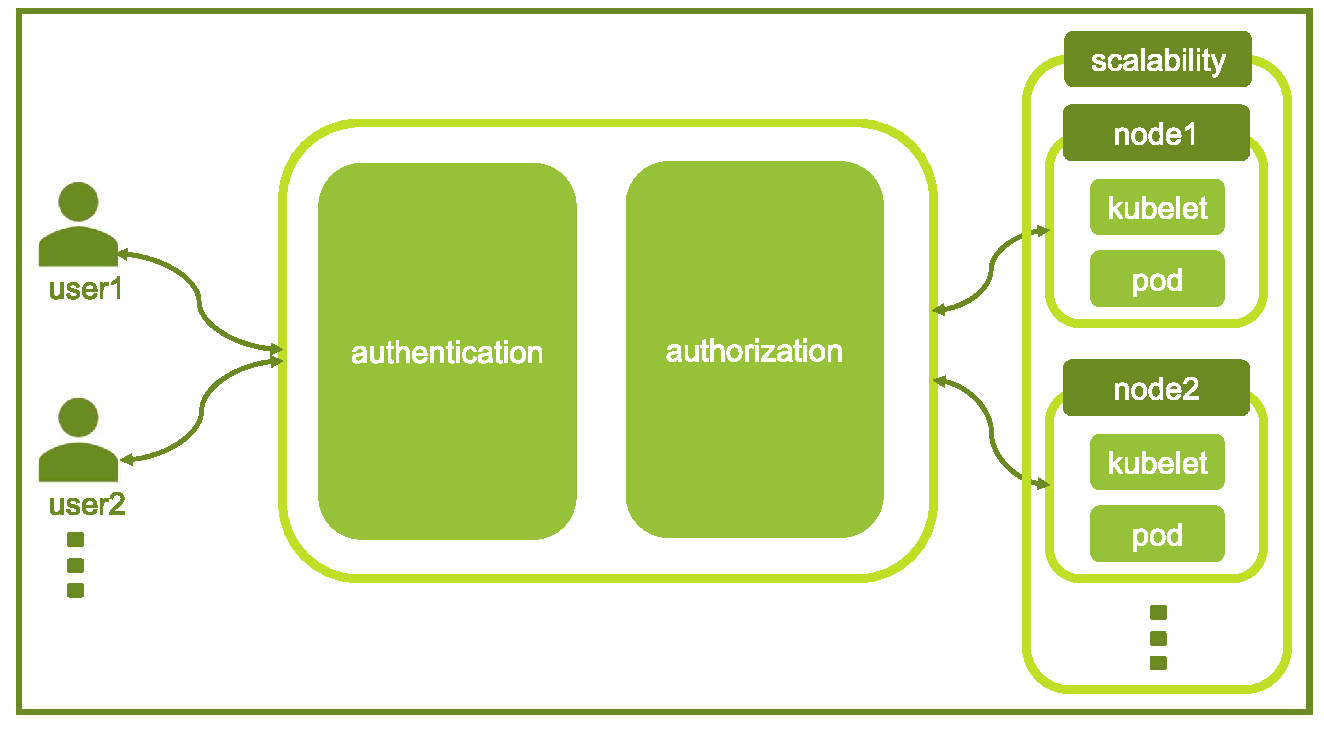
\includegraphics[width=16.88cm,height=9cm]{Thesis/Figures/title.pdf}
\end{textblock*}

\begin{textblock*}{13cm}[0,0](3.45cm, 2.9cm + 9cm + 9.2cm)
\singlespacing
\begin{table}[h!]
	\begin{tabular}{p{3.5cm}p{7cm}R{4.2cm}}
		Author: 	&	Muhammad Fahad Ali, 22995110\\
		& & \\
		Supervisor(s):		&	Prof. Dr.-Ing. Jörg Franke
            & &
                              &  Benedikt Scheffler, M.Sc.	& \\ 
		& & \\
                                    
		Submission date: 	&	30.10.2024 				& \\
		Processing time:	&	\BEARBEITUNGSZEIT\ months &
	\end{tabular}
\end{table}
\end{textblock*}

%\topmargin2cm
%\thispagestyle{empty}
%\renewcommand{\baselinestretch}{1.25}\normalsize
\mbox{ }

\newpage
\thispagestyle{empty}



			    % Deckblatt

	\chapter*{Declaration}
\thispagestyle{empty}
I hereby declare that I have written this thesis without outside help and without using any sources other than those indicated. This thesis has not been submitted in the same or a similar version to any other examination office and been accepted as part of an examination performance. All statements that have been adopted literally or paraphrased are marked as such.\\
\vspace{1.5cm}

Nürnberg, 30.09.2024\\[-5mm]
\hspace*{10.4cm}\rule[-0.3pt]{0.35\linewidth}{0.4pt}\\[0mm]
\hspace*{11.5cm}Muhammad Fahad Ali

%\newpage
\thispagestyle{empty}
\mbox{ }
\newpage			% Erklaerung, dass alles alleine gemacht wurde

        \chapter*{Abstract}
\thispagestyle{empty}

In today’s rapidly evolving technological landscape, cloud-native architectures have become essential for building secure, scalable and distributed applications. In this thesis we explores the implementation of a cloud-native architecture designed to address these key challenges, leveraging advanced tools and techniques to enhance security, scalability, and distributed computation.\cite{1}\\
A significant portion of this research focuses on implementing Role-Based Access Control \abk{RBAC}{Role-Based Access Control} in Kubernetes and automating the entire process. This approach ensures fine-grained access control and enhances the security of the Kubernetes environment\cite{2}. Additionally, the integration of ArgoCD with Keycloak for authentication is examined to enhance security.\\
To achieve scalability, we leverage Ray, a distributed execution framework that enables efficient autoscaling and hyperparameter optimization. Ray's core pillars are implemented to enhance computational efficiency and support distributed computation. This integration ensures that the system can dynamically scale resources based on workload demands, providing a flexible and resilient computing environment.


%\newpage
\thispagestyle{empty}
\mbox{ }
\newpage
        
	\frontmatter				% Roemische Seitennummerierung

	%\nopagebreak
	\cleardoublepage
	\currentpdfbookmark{Contents}{Contents}	% Lesezeichen fuer Inhaltsverzeichnis
	\tableofcontents			% Inhaltsverzeichnis
	
	

% Inhaltsverzeichnislayout
\setcounter{tocdepth}{3} % 3 Gliederungsebenen im Inhaltsverzeichnis

% Formatierung der Verzeichnisse im Inhaltsverzeichnis
\titlecontents{chapter}
[0em]	% Abstand linker Textrand bis Kapitelueberschriften
{}	% Textformatierung
{}	% Abstand und Nummerierung vor Kapitelueberschriften
{}
{\vzPunkte\contentspage} % Formatierung nach Titel bis zur Seitenzahl


% Define new list for code snippets
\newlistof{listingsnippets}{lol}{List of Code Snippets}


% Define how code snippets should appear in the list
\newcommand{\listingsnippet}[2]{
  \refstepcounter{listingsnippets} 
  \addcontentsline{lol}{listingsnippets}{\protect\numberline{\thelistingsnippets}#1}%
  \begin{tcolorbox}[colback=white, colframe=black, 
    boxrule=0.5mm, sharp corners=south, 
    bottomrule=0.5mm, toprule=0.5mm, left=0mm, right=0mm, coltitle=black]
    \begin{lstlisting}
#2
    \end{lstlisting}
  \end{tcolorbox}
  \vspace{-0.5\baselineskip}
  \begin{center} % Center the caption
    \textit{Code Snippet \thelistingsnippets: #1} 
  \end{center}
  \label{listingsnippet:\thelistingsnippets}
}



% Custom format for list of code snippets (optional)
\renewcommand{\cftlistingsnippetsleader}{\cftdotfill{\cftdotsep}} % Dotted lines in list


% Abbildungsverzeichnis
\cleardoublepage
\addtocontents{lof}{\vskip -0.35cm}
\renewcommand{\cftfigleader}{\vzPunkte}
\renewcommand{\cftfigindent}{0em}
\listoffigures%


% Tabellenverzeichnis
\cleardoublepage
\addtocontents{lot}{\vskip -0.35cm}
\renewcommand{\cfttableader}{\vzPunkte}
\renewcommand{\cfttabindent}{0em}
\listoftables%


\cleardoublepage
\listoflistingsnippets % Generates the list of code snippets
\addcontentsline{toc}{chapter}{List of Code Snippets} % Add the generated list to TOC

% Abkuerzungs- und Symbolverzeichnis
\cleardoublepage
\printnomenclature			% Abkürzungs- und Symbolverzeichnis


% Formatierung des Inhaltsverzeichnisses
\titlecontents{chapter}
[1em]	% Abstand linker Textrand bis Kapitelueberschriften
{\vspace{12pt}\bf}	% Textformatierung
{\contentslabel{1em}}	% Abstand und Nummerierung vor Kapitelueberschriften
{}
{\vzPunkte\contentspage\vspace{8pt}} % Formatierung nach Titel bis zur Seitenzahl

\titlecontents{section}
[2.79em] % Abstand linker Textrand bis Kapitelueberschriften
{} % Textformatierung
{\contentslabel{1.809em}} % Abstand und Nummerierung vor Kapitelueberschriften
{}
{\vzPunkte\contentspage} % Formatierung nach Titel bis zur Seitenzahl

\titlecontents{subsection}
[5.387em] % Abstand linker Textrand bis Kapitelueberschriften
{} % Textformatierung
{\contentslabel{3em}}% Abstand und Nummerierung vor Kapitelueberschriften
{}
{\vzPunkte\contentspage} % Formatierung nach Titel bis zur Seitenzahl

% Optional: Renaming Bibliography
%\renewcommand\bibname{References}


	\mainmatter				    % Arabische Seitennummerierung

	%%%%%%%%%%%%%%%%%%%%%%%%%%%%%%%%%%%%%%%%%%%%%%%%%%%%%%%%%%%%%%%%%%%%%%%%%%%%%%%%%%%%%%%%%%%%%%
	%%%%   FILL WITH OWN CONTENT                                                               %%%
	%%%%%%%%%%%%%%%%%%%%%%%%%%%%%%%%%%%%%%%%%%%%%%%%%%%%%%%%%%%%%%%%%%%%%%%%%%%%%%%%%%%%%%%%%%%%%%

%
%	The insertion of chapters is done here:
%

		\chapter[Introduction]{Introduction}
....



		%\chapter{Related Work}
\label{Kapitel_erste}
% Labels sind fuer Verknuepfungen im Text notwendig
\textbf{Notice: This template has not yet been fully translated into English. Please contact your supervisor if you have any questions regarding the formatting.}
\bigskip

Kapitel werden mit $\backslash\!chapter\left\{ Titel \right\}$ eingeführt.

Dann folgt das erste Kapitel....

\section{Subchapter}
Ein Unterkapitel wird mit $\backslash\!section\left\{ Titel \right\}$ bezeichnet.

Hier sollen einige weitere Beispiele folgen, wie Bilder, Tabellen und Formeln eingegeben werden.

Tabellen, wie Tabelle \ref{Tabelle_Beispiel} werden wie folgt eingefügt:

\begin{longtable}[c]{L{4cm}C{4cm}p{4cm}}%
	% Definition des Tabellenkopfes
	\caption{Beispiel-Tabelle}
	\label{Tabelle_Beispiel} \\
	\toprule
	\rowcolor{hellgrau}
	1. Spalte	(linksbündig)							&	2. Spalte	(horizontal zentriert)		&		3. Spalte (linksbündig, vertikal zentriert)\\ \midrule
	\endfirsthead % Erster Kopf zu Ende
	%
	% Definition des Tabellenkopfes auf den folgenden Seiten
	\caption*{Beispiel-Tabelle - Fortsetzung}\\
	\toprule
	\rowcolor{hellgrau}
	1. Spalte	(linksbündig)							&	2. Spalte	(horizontal zentriert)		&		3. Spalte (Blocksatz)\\ \midrule
	\endhead % Zweiter Kopf ist zu Ende
	%
	\multicolumn{3}{r}{Fortsetzung von \tab{Tabelle_Beispiel} auf der nächsten Seite}\\
	\endfoot
	\bottomrule
	%\multicolumn{3}{r}{} \\
	\endlastfoot
	% Ab hier folgt der Inhalt der Tabelle
	1. Zeile mit ein bisschen Inhalt zeigt den Unterschied	& Inhalte über mehrere Zeilen zeigen die Effekte & Text über mehrere Zeilen zeigt den Effekt \\ \midrule
	%
	2. Zeile	& Inhalte & Text \\ \midrule
	%
	usw.			& Inhalte & Text 
\end{longtable} 

Ein riesen Vorteil von \LaTeX\; ist die Formelumgebung. Damit diese durchgehend
nummeriert sind, werden diese wie folgt eingefügt, wobei die Gleichung
\begin{align}
	\label{Formel_Beispiel}
	x&=\sqrt[3]{\int \limits_{i=0}^{n} \frac{1}{\sqrt{a^2 + \frac{b^2}{x}}} \mbox{d}x}\\
	a^2+b^2 &= c^2
\end{align}

in den Textfluss eingearbeitet werden sollte. Es ist zu beachten, dass ebenfalls der Bezug zu Formel
\eqref{Formel_Beispiel} im Textfluss lesbar eingefügt sind.

Wenn z.B. das Bild \ref{Bild_Beispiel} eingefügt werden soll, passiert das wie
folgt:
% Bild einfuegen
\begin{figure}[ht!]
	\centering
 	
\includegraphics[width=0.4\textwidth]{LogoFAPS}
	\caption{Unser FAPS-Logo}
	\label{Bild_Beispiel}
\end{figure}

Für einen Eintrag in das Abkürzungsverzeichnis kann bei Verwendung von
Abkürzungen der Befehl $\backslash\!abk\left\{\text{\emph{ABK}}\right\}\left\{ausgeschriebene Bezeichnung\right\}$ verwendet werden. Es sollte
beachtet werden, dass das abzukürzende Wort vor Verwenden der Abkürzung immer
mindestens einmal ausgeschrieben ist.
Das kann dann wie folgt aussehen: Eine zweibuchstabige Abkürzung \abk{ZBA}{zweibuchstabige Abkürzung} ist eine dreibuchstabige Abkürzung \abk{DBA}{dreibuchstabige Abkürzung}.

Für mathematische Konstanten o.ä. funktioniert das auch. Die Gravitationskonstante $\const{g}$ erhält durch
den Befehl $\backslash\!abk\left\{\const{g}\right\}\left\{g\right\}\left\{Gravitationskonstante\right\}$ einen Eintrag im Abkürzungsverzeichnis. Dabei ist die zweite Klammer eine Sortierungshilfe für das Verzeichnis. Die Bezeichnung in der dritten Klammer kann für das Verzeichnis angepasst werden und erscheint nicht im Text. Ausgeführt sieht das dann so aus: \abk{$\const{g}$}{g}{Gravitationskonstante}. Auch griechische Buchstaben sind kein Problem, wie beispielsweise der \abk{$\eta$}{eta}{Wirkungsgrad} mit $\backslash\!abk\left\{\eta\right\}\left\{eta\right\}\left\{Wirkungsgrad\right\}$ beschrieben wird.

Im Literaturverzeichnis sind alle Quellen anzugeben. Des Weiteren kann darin für weitere Informationen geschmökert werden.
Zitieren funktioniert mit dem Befehl $\backslash\!cite\left\{ Buch\;etc.\right\}$. Das ergibt dann z.B. \cite{Resetarics.2009}. Die Literaturliste kann als BiBTeX-Datei aus Citavi exportiert werden. Dabei tauchen dann im Text nur die Quellen auf, welche auch tatsächlich zitiert wurden.

\subsection{Sub-subchapter}
In einer Arbeit sollten die Kapitel und Abschnitte nicht tiefer als die dritte
Ebene sein. Zumindest tauchen weitere Überschriften nicht im Inhaltsverzeichnis auf.

Als Ergänzung wird im Folgenden noch aufgezeigt, wie zwei Bilder nebeneinander
dargestellt werden. Referenziert werden diese Bilder analog zu vorher. Beispielsweise zeigt Abbildung \ref{Bild_Beispiel_zwei_Bilder_links} eine Roboterhand mit einem Apfel, wobei in Abbildung \ref{Bild_Beispiel_zwei_Bilder_rechts} wiedermal das FAPS-Logo zu sehen ist. Zu beachten ist, dass nur die Hauptbeschriftung im Abbildungsverzeichnis auftaucht. Diese ist oft auch einfach nur eine Kurzform.

\begin{figure}[ht!]

% Breite darf maximal 0.49*\textwidth sein, wobei die Hoehe der zwei Bilder
% gleich sein sollte
\newcommand{\pictureheight}{5cm}

	\begin{minipage}[c]{.49\textwidth}
		\centering
		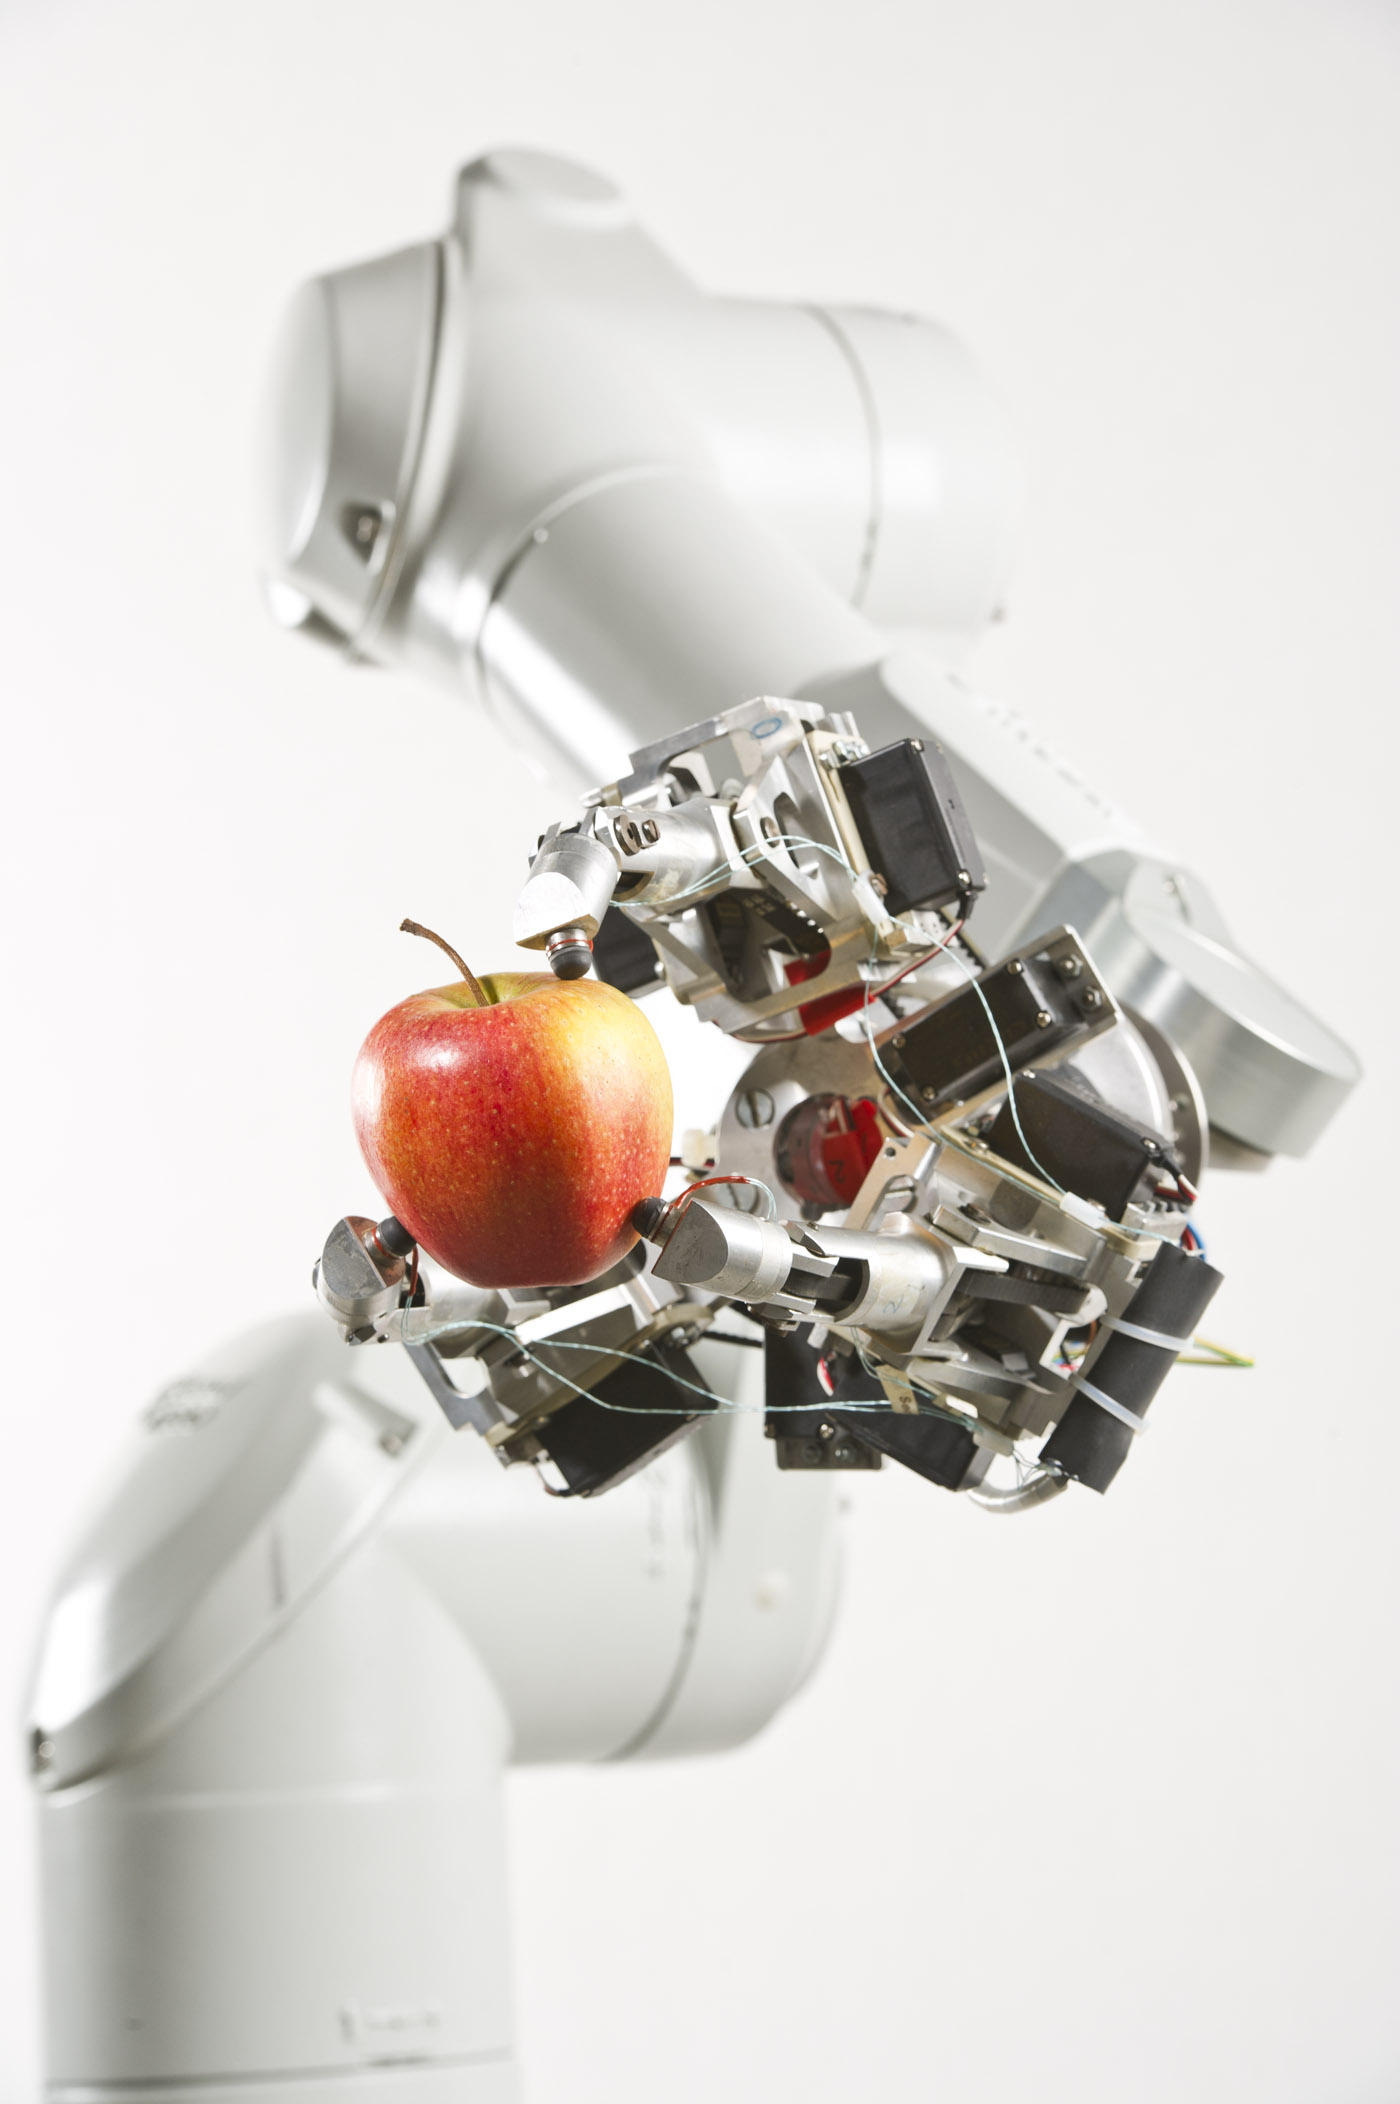
\includegraphics[height=\pictureheight]{Biomechgreifer.jpg}
		\subcaption{Roboterhand mit Apfel}
		\label{Bild_Beispiel_zwei_Bilder_links}
	\end{minipage}
%	
	\begin{minipage}[c]{.49\textwidth}
        \centering
		
\includegraphics[height=\pictureheight]{LogoFAPS}
		\subcaption{FAPS-Logo}
		\label{Bild_Beispiel_zwei_Bilder_rechts}
	\end{minipage}
    	
    	\caption[Zwei Bilder nebeneinander]{Hier sind zwei Bilder zu sehen, welche nebeneinander angeordnet sind.}
	\label{Bild_Beispiel_zwei_Bilder}

\end{figure}

Auflistungen werden wie folgt gemacht:
\begin{itemize}
	\item Das wird der erste Stichpunkt
	\item Ein zweiter Stichpunkt
	
	\begin{itemize}
		\item Das ist die nächste Ebene
	\end{itemize}
	
\end{itemize}

		\chapter{Proposed Approach}
...

		% Folgender Befehl erzwingt an entsprechender Stelle einen Seitenumbruch
		% Bei einer Seite bitte ausblenden
%		\addtocontents{toc}{\protect\newpage}

		\chapter{Summary and Outlook}
....

	%%%%%%%%%%%%%%%%%%%%%%%%%%%%%%%%%%%%%%%%%%%%%%%%%%%%%%%%%%%%%%%%%%%%%%%%%%%%%%%%%%%%%%%%%%%%%%
	%%%%   DO NOT CHANGE                                                                       %%%
	%%%%%%%%%%%%%%%%%%%%%%%%%%%%%%%%%%%%%%%%%%%%%%%%%%%%%%%%%%%%%%%%%%%%%%%%%%%%%%%%%%%%%%%%%%%%%%
	
	\cleardoublepage
\thispagestyle{plain}

% Inhaltsverzeichnis-Eintrag
\titlecontents{chapter}
[0em]
{\vspace{12pt}}
{\contentslabel{1em}}
{}
{\vzPunkte\contentspage}

% Code für Linksbuendigkeit der Klammern 
\makeatletter 
	\renewcommand*{\@biblabel}[1]{\makebox[\labelwidth][l]{[#1]}}
\makeatother

% Label-Width - Eintrag entspricht max. Anzahl an Ziffern
\setbiblabelwidth{99}

% Literaturverzeichnis Stil
% 2023/06/23: changes bibliography style to a English one
\bibliographystyle{ieeetr}
%	Pfad:		C:\Program Files (x86)\MiKTeX 2.9\miktex\bin\bibtex.exe
%	Argumente:	"%bm"}
% Am besten aus Citavi exportieren
\bibliography{Verzeichnis_Literatur}


%%%%%% Extra Verzeichnisse %%%%%
\cleardoublepage
\thispagestyle{plain}

% Inhaltsverzeichnis-Eintrag
\titlecontents{chapter}
[0em]
{}
{\contentslabel{1em}}
{}
{\vzPunkte\contentspage}

%%%%% Quellenverzeichnis %%%%%%

% Label-Width - Eintrag entspricht max. Anzahl an Ziffern
\setbiblabelwidth{9}


%	Postprozessor:
		%Anwendung: 	bibtex.exe
		%Argumente:		Q



%% Layout Inhaltsverzeichnis wiederherstellen
%\input{Format_ToC}	% Literaturverzeichnis (BibTeX)	
	
	\appendix										% Beginn des Anhangs
	% Bezeichnungen und Nummerierungsstile
\renewcommand{\chaptername}{Anhang}
% \renewcommand{\theequation}{\Alph{section}.\arabic{equation}}
\renewcommand{\theequation}{\Alph{chapter}.\arabic{equation}}
\renewcommand{\thetable}{\Alph{chapter}.\arabic{table}}
\renewcommand{\thefigure}{\Alph{chapter}.\arabic{figure}}


% Inhaltsverzeichnislayout fuer 'Anhang'
\titlecontents{chapter}
[1em]	% Abstand linker Textrand bis Kapitelueberschriften
{}	% Textformatierung
{\contentslabel{1em}}	% Abstand und Nummerierung vor Kapitelueberschriften
{}
{\vzPunkte\contentspage} % Formatierung nach Titel bis zur Seitenzahl


% Erscheinen von 'Anhang' im Inhaltsverzeichnis
%\addtocontents{toc}{\protect\contentsline{chapter}{Anhang}{}{}}

				% Formatierung des Anhangs
		%
	%%%%%%%%%%%%%%%%%%%%%%%%%%%%%%%%%%%%%%%%%%%%%%%%%%%%%%%%%%%%%%%%%%%%%%%%%%%%%%%%%%%%%%%%%%%%%%
	%%%%   FILL WITH OWN CONTENT, IF APPLICABLE                                                %%%
	%%%%%%%%%%%%%%%%%%%%%%%%%%%%%%%%%%%%%%%%%%%%%%%%%%%%%%%%%%%%%%%%%%%%%%%%%%%%%%%%%%%%%%%%%%%%%%

%
%	The insertion of attachments is done here:
%

		\chapter{Appendix}
\label{A_Appendix}
% 
Hier kommt das hin, was in der Ausführung für Unübersichtlichkeit gesorgt
hätte...

		
		%\includepdf[pages=1-2, scale=0.75, pagecommand={\thispagestyle{fancy}}, offset=0.5cm 1.5cm]{Test_Anhang.pdf}
		%\cleardoublepage
		
		
	%%%%%%%%%%%%%%%%%%%%%%%%%%%%%%%%%%%%%%%%%%%%%%%%%%%%%%%%%%%%%%%%%%%%%%%%%%%%%%%%%%%%%%%%%%%%%%
	%%%%  CV IF DESIRED (adjust the command \Lebenslauf above accordingly)                     %%%
	%%%%%%%%%%%%%%%%%%%%%%%%%%%%%%%%%%%%%%%%%%%%%%%%%%%%%%%%%%%%%%%%%%%%%%%%%%%%%%%%%%%%%%%%%%%%%%
	
	\ifthenelse{\equal{\Lebenslauf}{CV}}{
		\currentpdfbookmark{Curriculum Vitae}{Curriculum Vitae}	% Lesezeichen fuer Lebenslauf
		\thispagestyle{empty}
		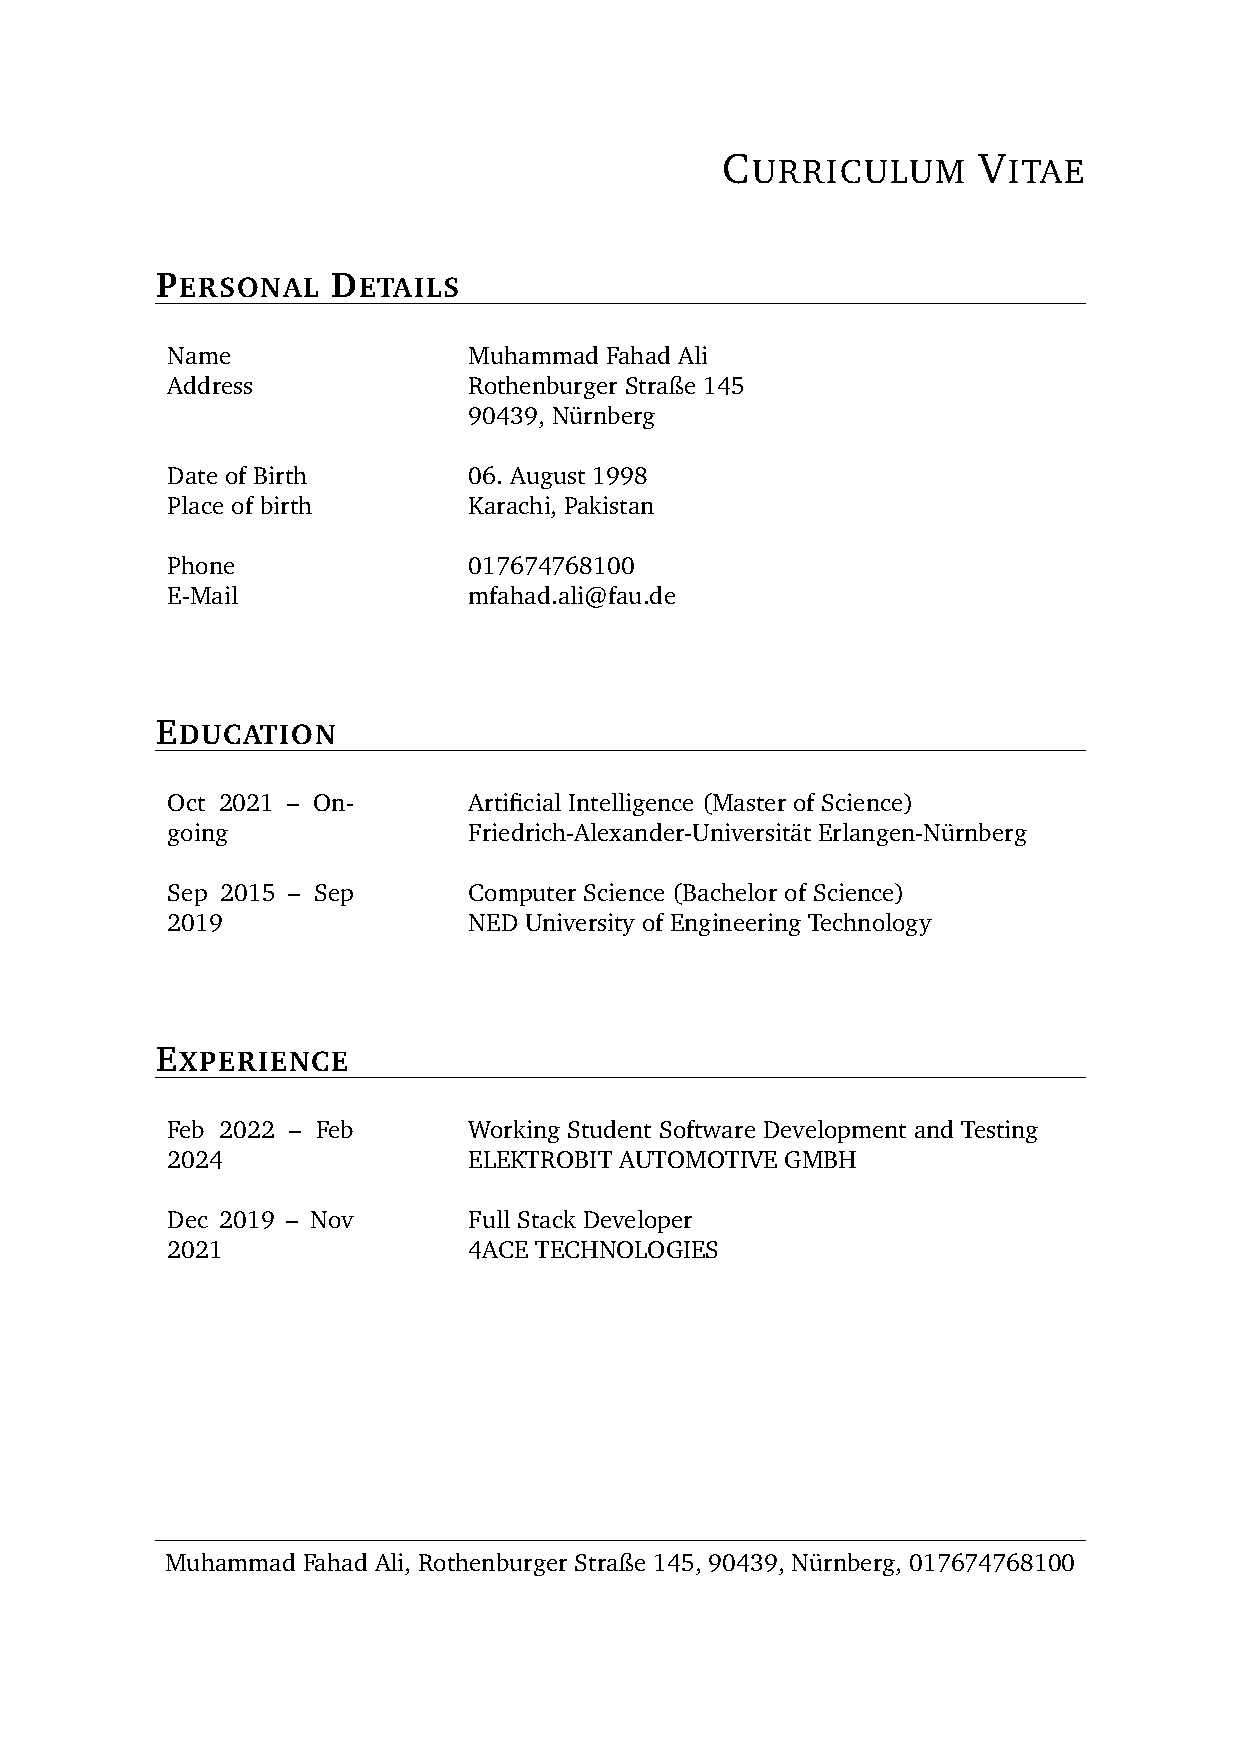
\includepdf[pages={1},offset= {0.5cm, -0.5cm}]{CurriculumVitae.pdf}
		\cleardoublepage
	}{}
 
% 2023/06/23: added the following line for bug fix regarding abbreviations
 \printnomenclature
\end{document}

